\section{The Big Picture}
\begin{frame}{The Big Picture}{grosses Projekt}
 \begin{description}
  \item[Gegeben] Eine grosse Anzahl {\em source} Files
  \item[Gesucht] 2 Files:
   \begin{itemize}
    \item das {\Large Image}
    \item der {\em Devicetree}
   \end{itemize}
  \item[L�sung] Klassisches Verfahren
  \begin{itemize}
   \item Toolchain
   \item Makefile
  \end{itemize}
 \end{description}
\end{frame}

\begin{frame}{Die Schichten}
 \begin{center}
  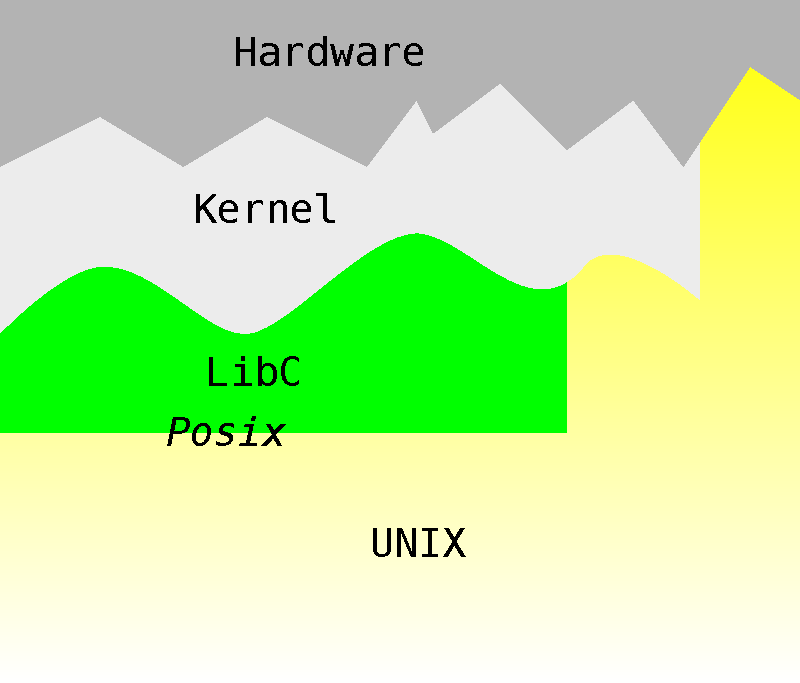
\includegraphics[width=0.75\textwidth]{layers.pdf}
 \end{center}
\end{frame}

\begin{frame}{Kernel}{Grosses Projekt}
\begin{block}{Was ist einfach ?}
 \begin{itemize}
  \item \kernel h�ngt nicht von anderen Software Komponenten ab
  \begin{itemize}
   \item stand alone
  \end{itemize}
  \item Braucht nur \cod{make} und {\em toolchain}
 \end{itemize}
\end{block}
\begin{block}{Was ist schwierig ?}
 \begin{itemize}
  \item Konfiguration
  \begin{itemize}
   \item Wahl der richtigen {\em source} Files f�r das {\Large Image}
  \end{itemize}
 \end{itemize}
\end{block}
\end{frame}
